\documentclass{article}

\usepackage{fullpage}
\usepackage{graphicx}

\begin{document}

\title{Approximating Functions for Grid Domains}
\author{Danny Zhu (dannyz) \and Yuzi Nakamura (ynakamur) \and Ben Humberston (bhumbers)}

\maketitle

\section{Introduction}

Approximate computing is a method of computation that sacrifices accuracy to save computation time and energy. For certain problems, full exactness may not be necessary, and the savings gained in battery life, execution time, or power costs may be worth more than the loss in accuracy. In particular, we are inspired by code for the RoboCup Small-Size League, where speed in decision-making trades off with the optimality of the final decision: a team's AI must be ready to send out commands regularly at 60 hertz, and it is important to make some decision at all, even if a robot is positioned at a slightly suboptimal location. Approximate compilation is a promising way of implementing approximate computation that can be done on current machines.

In this project, we take  C functions of a particular signature and compile them into various approximators (also C functions, with the same function signature). We then analyze them to determine the speedup and how well they approximate the original.

\section{Related Work}
In tandem with the renewed focus on parallel computing, interest in general-purpose approximate computing has increased recently in response to decelerating efficiency gains for traditional scalar microprocessors. Techniques in approximate compilation automatically produce inexact yet more efficient versions of programmer-specified ``approximable'' code regions or data structures. An approximating compiler is thus responsible for encapsulating the low-level implementation of approximated code derived from the original source code. Programmers' input over how the approximation is implemented may only be binary (e.g., annotating some functions as ``approximable'', as in \cite{Esmaeilzadeh12}), or they may be given finer-grained control over the trade-off between accuracy and speedup of the approximation, as in the quality programmable machine instructions from \cite{Venkataramani13}.

\cite{Agarwal09} introduces the SpeedPress compiler and SpeedGuard runtime which make use of an approximate compilation strategy that they term ``code perforation''. This strategy selectively drops iterations from long-lasting loops based on the current value of a user-defined quality metric. It has the advantage of allowing a computation to be dynamically retargeted for either realtime performance or accuracy, a useful property for time-critical systems.

Although our project is restricted to software approximation schemes, our primary motivation comes from \cite{Esmaeilzadeh12}, which presents a framework for offloading C++ function calls suitable for approximation to a programmable neural processing unit (NPU). Akin to graphics processing units (GPUs), which are used for accelerating raster graphic operations, the NPU is a computational accelerator designed to simulate neural network computations using decreased power and faster execution than is possible using a general-purpose CPU. \cite{Amant14} builds on this approach with additional insights on compiling for analog circuit NPUs. The compiler is given a model of the restrictions of analog network computations (limited precision, non-ideal activation functions, and restrictions on network topologies) and generates function-approximating networks accordingly.

An alternative to marking specific code sections or functions as ``approximable'' is to instead label data items as either precise or approximate, as in the ``EnerJ'' extension to Java from \cite{Sampson11}. Users of EnerJ may set annotations for approximate data in a manner similar to constant data qualifiers. The compiler statically enforces restrictions on data flow from approximate to precise containers unless the user explicitly permits it.

\section{Method}

We focused on a particular class of functions to approximate: those which take a list of doubles and generate a two-dimensional array of doubles as output. That corresponds to the following C signature, to which the target functions must conform:

\begin{verbatim}
        void f(int n_inst, double* input, int inputLen,
               double* output, int outputRows, int outputCols)
\end{verbatim}
where:
\begin{itemize}
\item {\tt n\_inst} is the number of input vectors to read and output grids to write;
\item {\tt input} is a pointer to the input values;
\item {\tt inputLen} is the number of features within each input vector;
\item {\tt output} is a pointer to the output matrix, which the function will fill with values; and
\item {\tt outputRows} and {\tt outputCols} specify the dimension of the output grids.
\end{itemize}

The reason for focusing on grid-structured outputs, rather than general lists of doubles, was the idea that we would be able to exploit properties such as continuity of the target function to improve the quality of approximations. Due to time constraints, we did not implement any such measures in our approximators, though we did rely on it for a gradient-based measure of closeness of fit.

We implemented a compilation framework in Python. The main program is given a target C file and function and a means of generating inputs for it. It then takes a set of generated inputs, along with the corresponding outputs from the function, and passes them to the various approximators. Each approximator uses some machine learning model to learn parameters mapping from the given inputs to the given outputs. It then generates a new C file containing a function with the same signature as the original, but whose body uses the learned parameters to execute the machine learning model. A diagram of this system is given in figure~\ref{fig:system}.

\begin{figure}
  \centering
  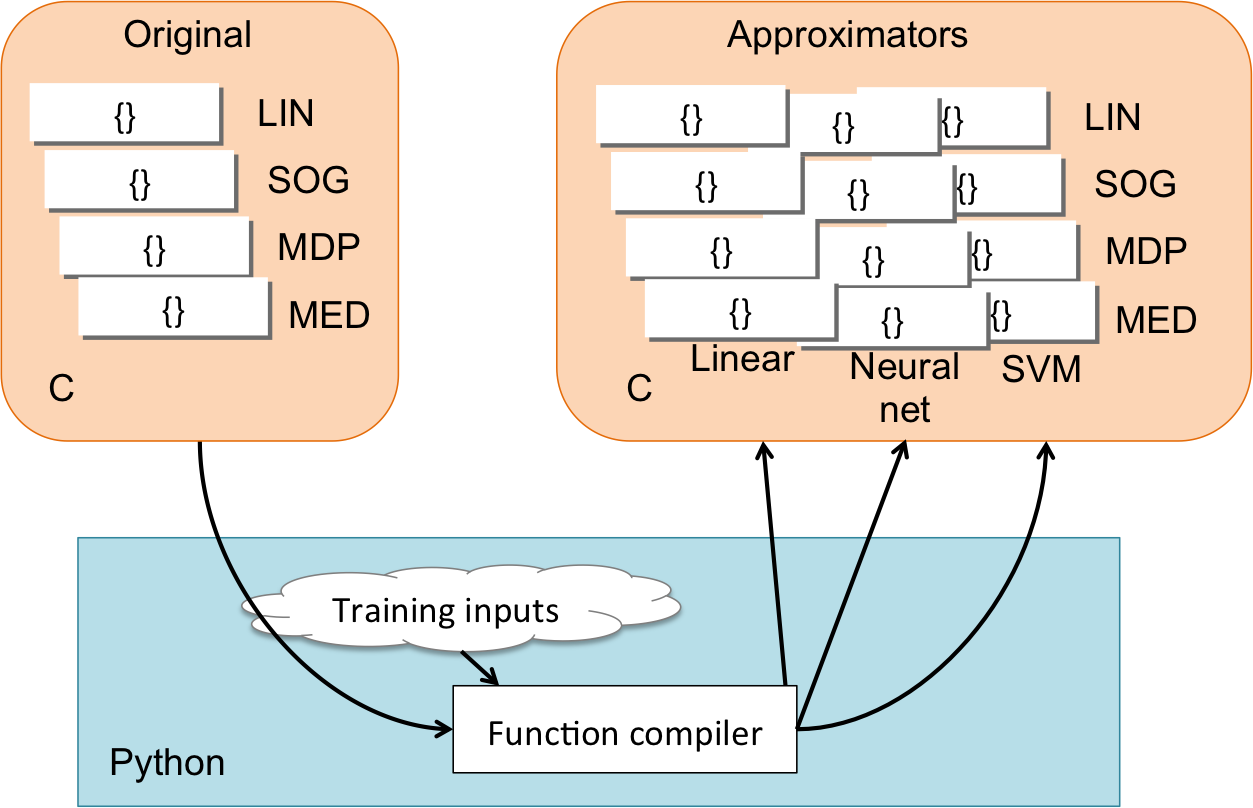
\includegraphics[width=4in]{images/diagram.png}
  \caption{System diagram: Our approximation compiler evaluates functions on various inputs and uses the results to train approximators. It then implements these approximators as C functions.}
  \label{fig:system}
\end{figure}

\subsection{Approximators}

\subsubsection{Linear regression}
This approximates the original function by assuming the function's value at each grid location to be a linear combination of all the input features. The weights defining the combinations are independent across locations. The approximation is learned using scikit-learn's linear model package, and the approximator outputs the weights and the simple code that evaluates the linear function using those weights to a file.

\subsubsection{Neural networks}

Similar to \cite{Esmaeilzadeh12}, we used a neural network to approximate functions. Neural networks are often used for function approximation; their nonlinear nature means that with enough nodes and training data, any function can be approximated to arbitrary precision.

We used FANN (the Fast Artificial Neural Network library) to learn the networks; in particular, we used its cascading mode, which uses the Cascade2 algorithm~\cite{fahlman} to build up the structure of the output neural net one node at a time, rather than having to specify a topology at the beginning. The algorithm also chooses an individual activation function and parameters for each node. This results in a much smaller final network than we could achieved with a fixed topology, which considerably reduces the time needed for evaluation, though it does increase the time needed for training.

The cascade method generates a network in which each hidden node has a connection from all input nodes and to all later-added hidden nodes, as well as all output nodes. This multi-layered structure allows for a rich connection structure with relatively few nodes, which gives the network expressivity without a high evaluation cost.

\subsubsection{SVM}

Support vector machines (SVMs), though usually used for classification, can be used for regression (in which case the technique is often referred to as ``support vector regression'' (SVR)). With nonlinear kernels, SVMs are capable of replicating a wide variety of functions. For the kernel function, we chose Gaussian radial basis functions, which are commonly used due to their versatility and small number of hyperparameters. Since SVMs have a one-dimensional output, we trained an independent SVM for each grid location.

Due to the importance of the $C$ and $\gamma$ hyperparameters for good performance, we also performed cross-validation for those parameters. We designated a set of values for $C$ and for $\gamma$; for each training set, we used a subset of the data to train a separate grid of SVMs for each possible pair of values, tested each grid on the remaining training data, and chose the one with the best score as the final trained regressor.

\section{Evaluation}

\subsection{Input Functions}

Our project was originally intended to be tested against inputs from a RoboCup planner agent, which would involve evaluating the utility of passing the ball to certain locations on the play field given the current state of the world (the locations and velocities of the robots and ball). However, it became apparent that it would be feasible neither to support the complex C++ function calls used in that code base nor to isolate an interesting problem that could be expressed independently of the main RoboCup code.

Instead, we evaluated several other problem domains which stand in for typical problems that face a robotic agent. Each of the problems accepts a vector of input values and outputs a two-dimensional grid of values. The size of the input vector and output grid must be fixed when generating an approximator.

\begin{itemize}
\item \textbf{Linear (LIN)} A basic problem type where each output grid value is a linear combination of the its grid coordinates. That is, the output value at grid location $(x, y)$ is $v = \alpha x + \beta y$, where the linear coefficients $\alpha$ and $\beta$ are constant over the whole grid and are used as the features for the approximators.

\item \textbf{Sum of Gaussians (SOG)} The output of a function of this type is the sum of one or more Gaussian basis functions placed randomly on the grid. While calculating this function is quite rapid even without approximation, the terrain that it generates presents good challenges for approximators, as it is non-linear in the function inputs.

\item \textbf{Markov decision process (MDP)} The output of problems of this type is the solution to value iteration for a Markov decision process problem instance defined over a square grid, emulating the planning of a robotic agent. The agent's state is a grid position $(x, y)$ and it may move deterministically in the four cardinal directions. One or more states are assigned a randomized reward value in the range $[0, 1]$. The computation cost of value iteration increases quickly for discount factors near unity and large grid state spaces, but it permits some imprecision in the computed values per state, as long as topological features of the output are preserved. This makes it a prime candidate domain for approximation.

\item \textbf{Median filter (MED)} A median filter is used in imaging processing applications to remove noisy pixels; however, performance degrades quickly for large filter window sizes. This function applies a median filter to a 2D input image with a filter window size of $7 \times 7$ pixels. While \cite{Esmaeilzadeh12} tested image filter approximations only at the per-pixel level, our approximators operate on pairs of two-dimensional input and output image patches (in order to keep the dimensionality of the approximation tractable, we limit the input and output images $20 \times 20$ pixels).
\end{itemize}

Note that we also considered the possibility of implementing an approximator scheme based on \textit{lookup tables}. However, we eliminated them as a viable option for our purposes, as their memory cost is intractable for the high dimensionality of our function inputs and outputs.

\subsection{Metrics}

\subsubsection{Error Metrics}
We use two metrics to evaluate the quality of each approximator: the \textit{absolute} and \textit{gradient} root-mean-square errors (RMSE).

The absolute RMSE metric simply measures the element-wise error for each output grid entry relative to the original function output, averaged over all test cases. This is a reasonable metric for general accuracy but doesn't impose any cost for approximators that fail to preserve topological features of the original output grids.

The gradient RMSE measures errors in the finite-difference gradient in the vertical and horizontal directions on the output grid, averaged over all test cases. Maintaining the gradient of the original function is desirable in order to preserve the local topology of the original function output.
\subsubsection{Performance Metrics}
In addition to output accuracy, we also evaluate approximators based on their execution performance, both in terms of compilation time and runtime speed. For the runtime measure, in addition to timing-based evaluation, we use Valgrind's ``callgrind'' tool to count dynamic instruction executions while calling approximated functions. We chose this tool rather than using llvm's interpreter for profiling as it also captures instructions executed in external libraries used by the approximators in addition to instructions directly generated from the approximator source.

\section{Results}

For each of the LIN, SOG, and MDP problem types, the approximators were trained on a set of 50 function input/output pairs and their quality was evaluated on a separate set of 50 test pairs. The output grids were of size $30 \times 30$ for LIN, SOG, and MDP problem domains and size $20 \times 20$ for the MED problem (the image chunk size).

Figure \ref{fig-pictures} shows a visual comparison of the results of running the original function and the three approximators on various test inputs for each of the problems. These images demonstrate that all three approximators generally do a good job of preserving global maxima/minima, and that neural networks and SVMs do a better job of approximating the original than linear regression.

\begin{figure}
  \centering
  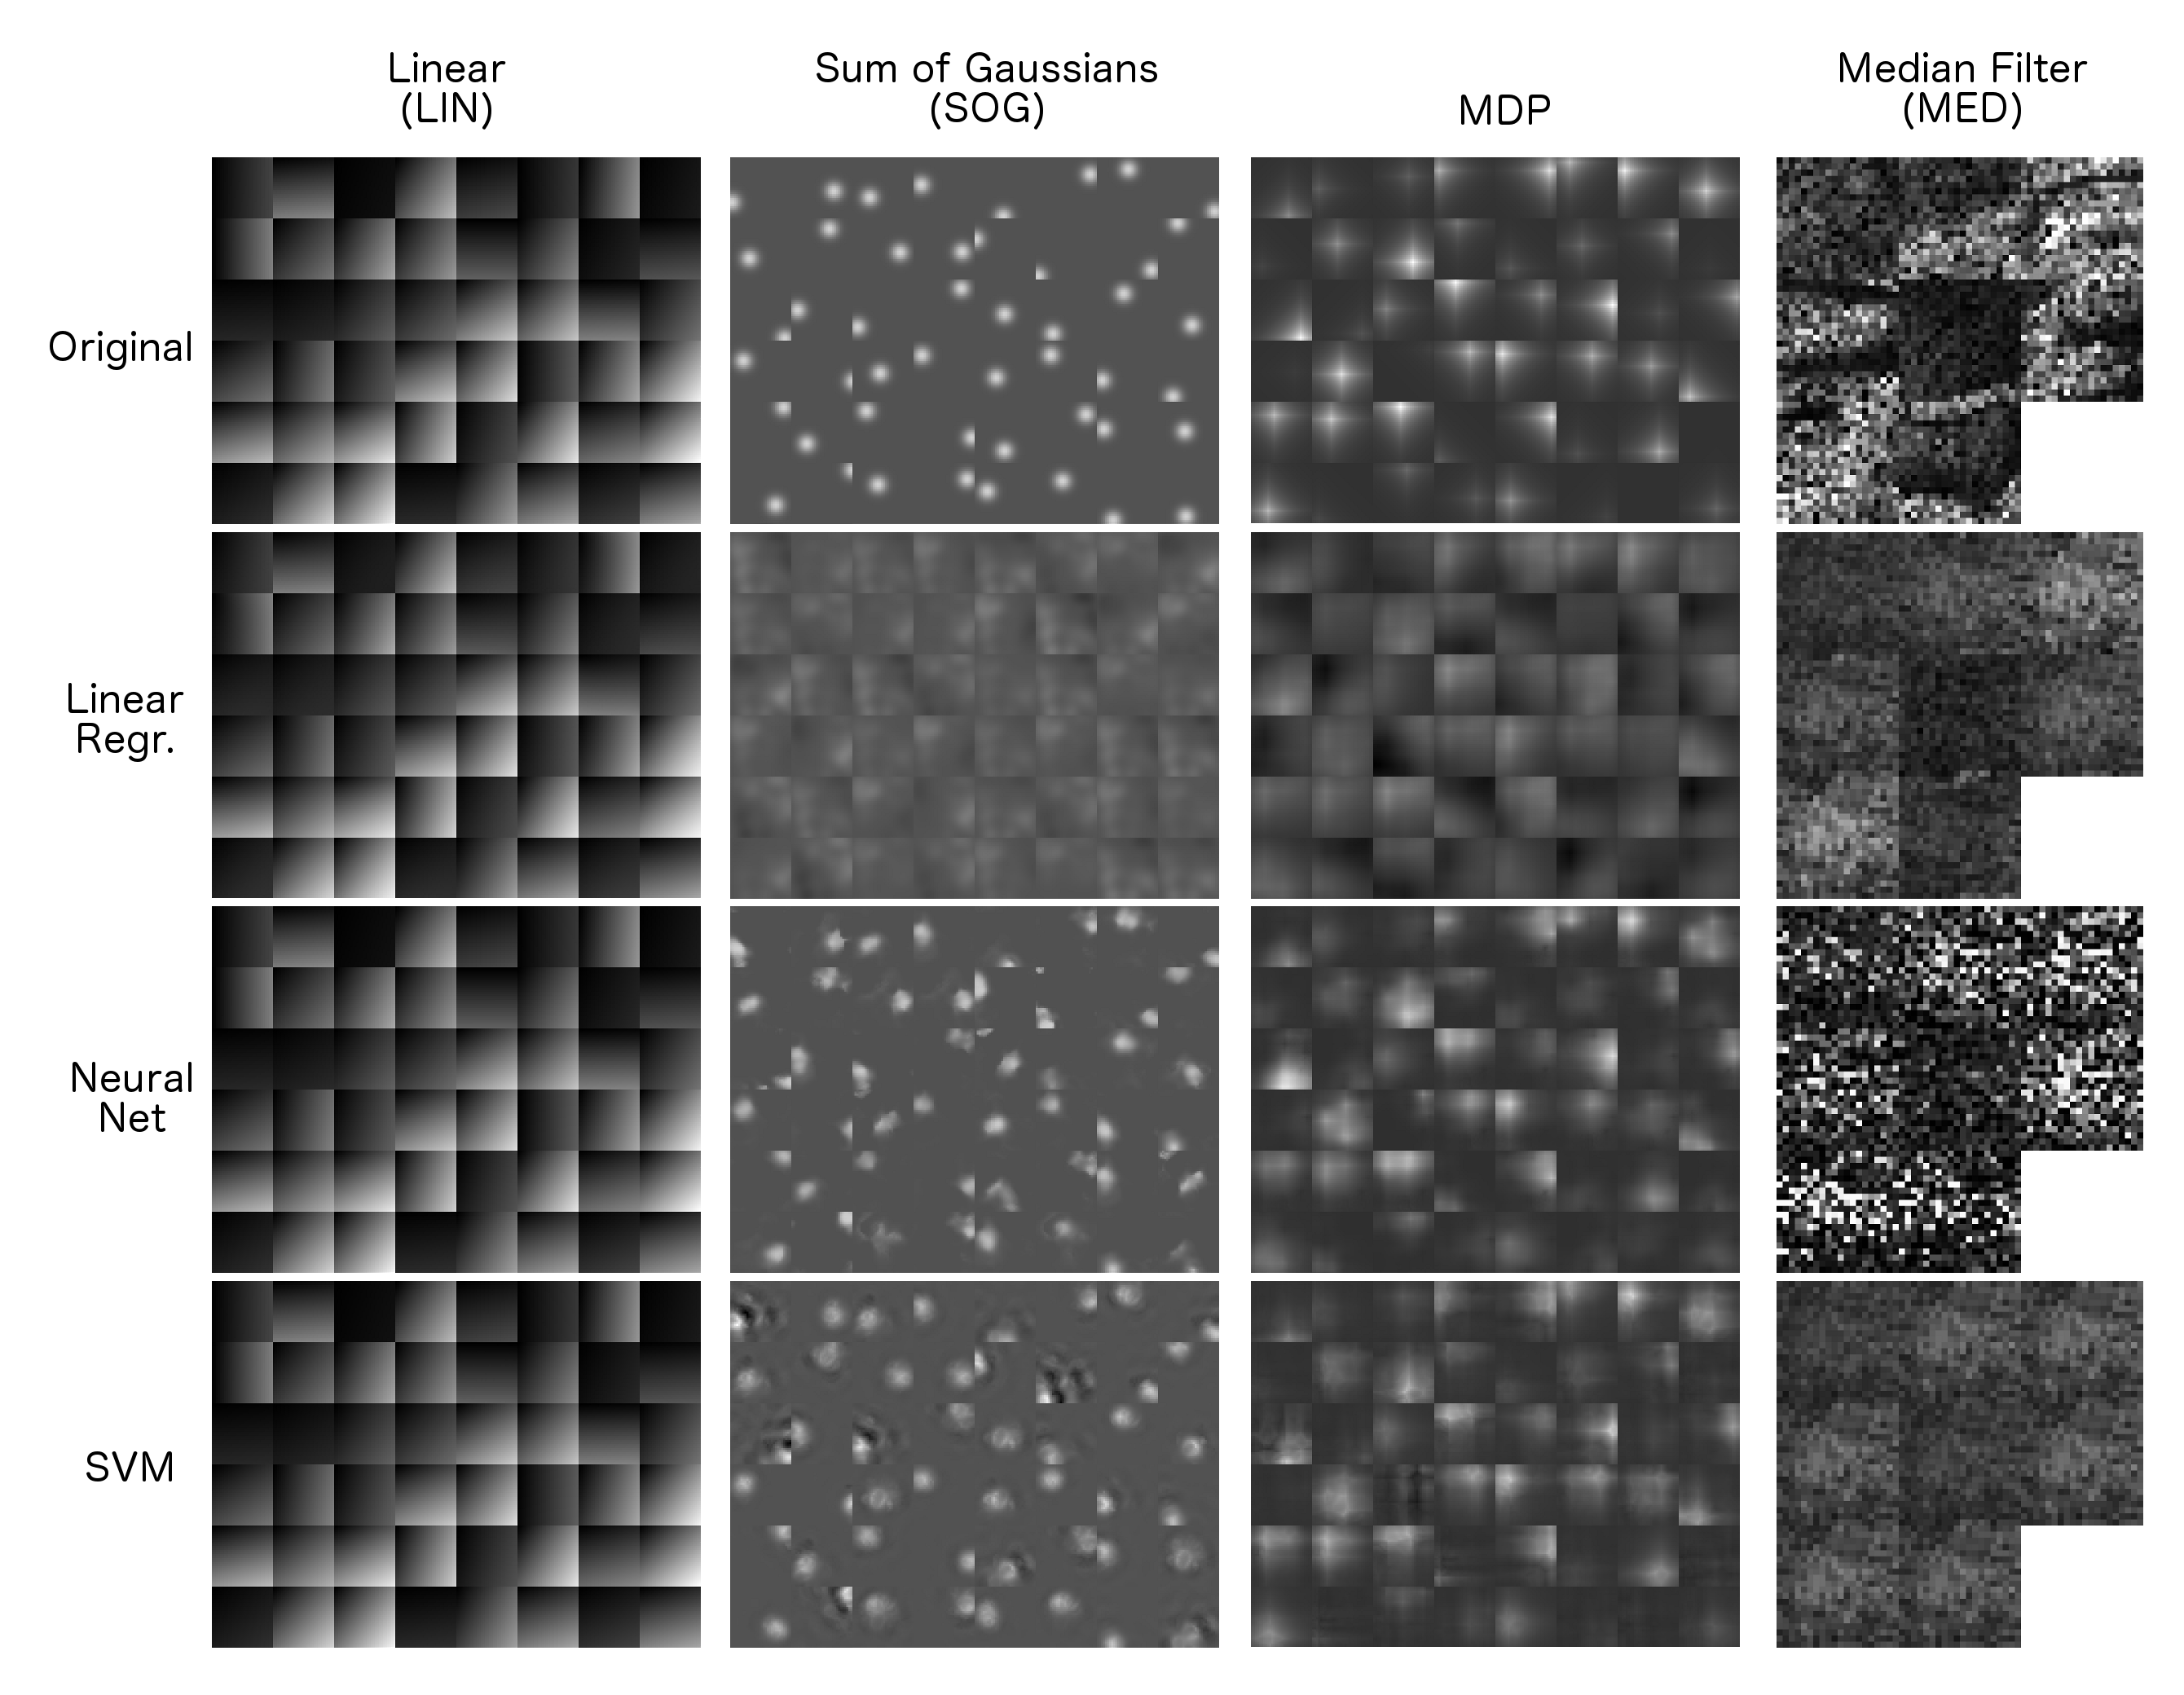
\includegraphics[width=6.3in]{images/results.png}
  \caption{Visual results comparison. The images above each contain a selection of test outputs i.e. the 2-D output generated by a function or function approximation from an input drawn from the test set. Row 1 therefore shows the results of running the original algorithms on typical function inputs, and the next three rows demonstrate the answers generated by the approximations on the same inputs. As you can see, for the linear problem, all approximations very closely resemble the original. Neural networks and SVMs do well for the sum of Gaussians and MDP problems as well, while linear regression does poorly but at least captures the location of the maximum. For the median filter, all three approximations generally resemble the original, but how well they approximate the original, even with this visual aid, is difficult to determine.}
  \label{fig-pictures}
\end{figure}
% Tables! Graphs! Pictures!

\subsection{Accuracy}

The absolute RMSE for our test suite is shown in Figure~\ref{fig:results_absolute_rmse}. All the approximators function well for the trivial LIN problem type, while the more advanced neural network and SVM models have the advantage over a simple linear approximator for the complex terrains generated by the sum-over-Gaussians and MDP problem types. However, on the median filter problem set (far right), there is no apparent gain from using these advanced approximators over the linear model. Note that the relationship between the inputs and outputs for the median filter problem type is different from that in the SOG and MDP problems; its input, consisting of an image patch and kernel size parameters, is of much higher dimensionality than the latter two types.


\begin{figure}
  \centering
  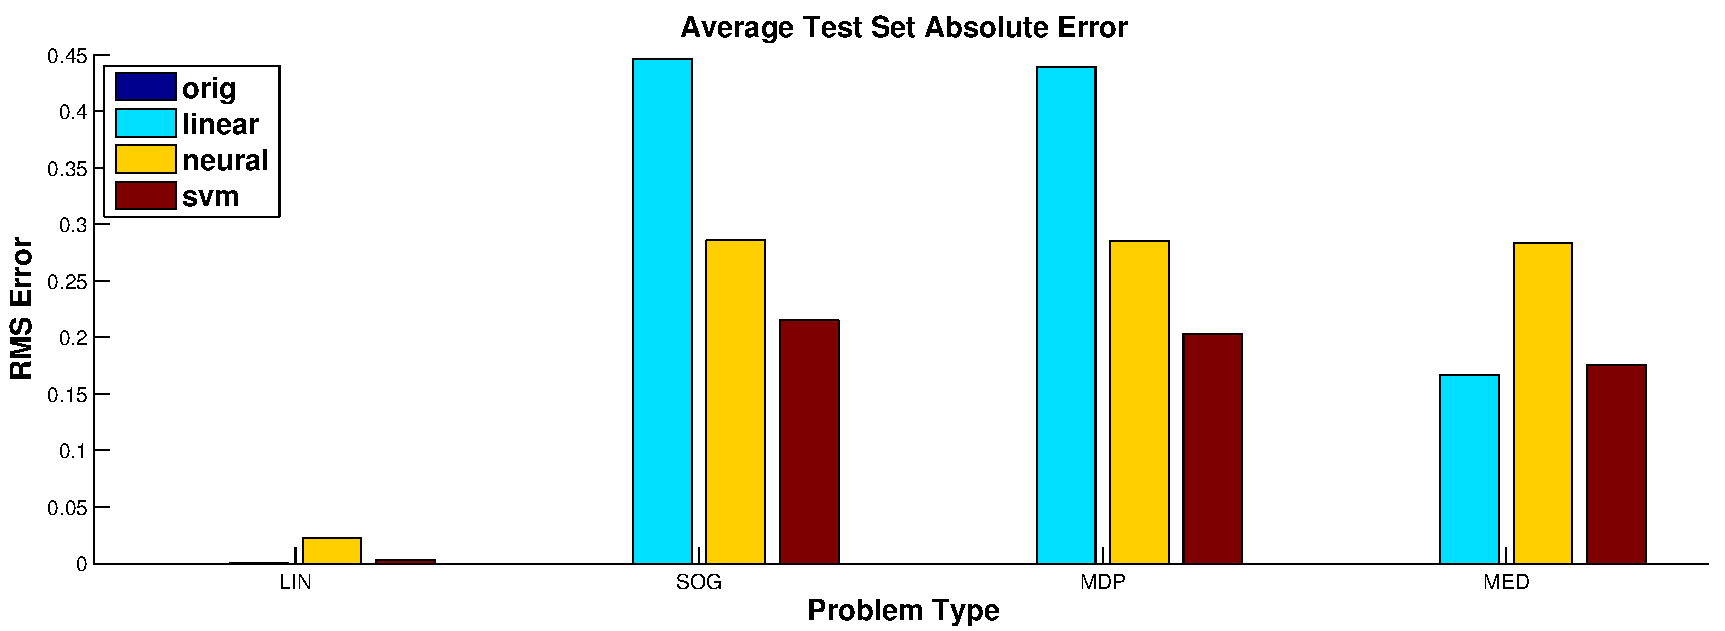
\includegraphics[width=0.8\textwidth]{images/results_rmse}
  \caption{Average absolute error by approximation strategy for each of our input function domains.}
  \label{fig:results_absolute_rmse}
\end{figure}

We provide the gradient RMSE for our test suite in Figure~\ref{fig:results_grad_rmse}. As with the absolute RMSE, all approximators handle well the trivial LIN problem type. The results on the more challenging sets are mixed, with no clear advantage to any approximator type.

Based on visual inspection, the neural network and SVM approximators seem to show better topology preservation than the linear approximator, but we believe that another topological metric may be necessary to capture this apparent qualitative difference.

\begin{figure}
  \centering
  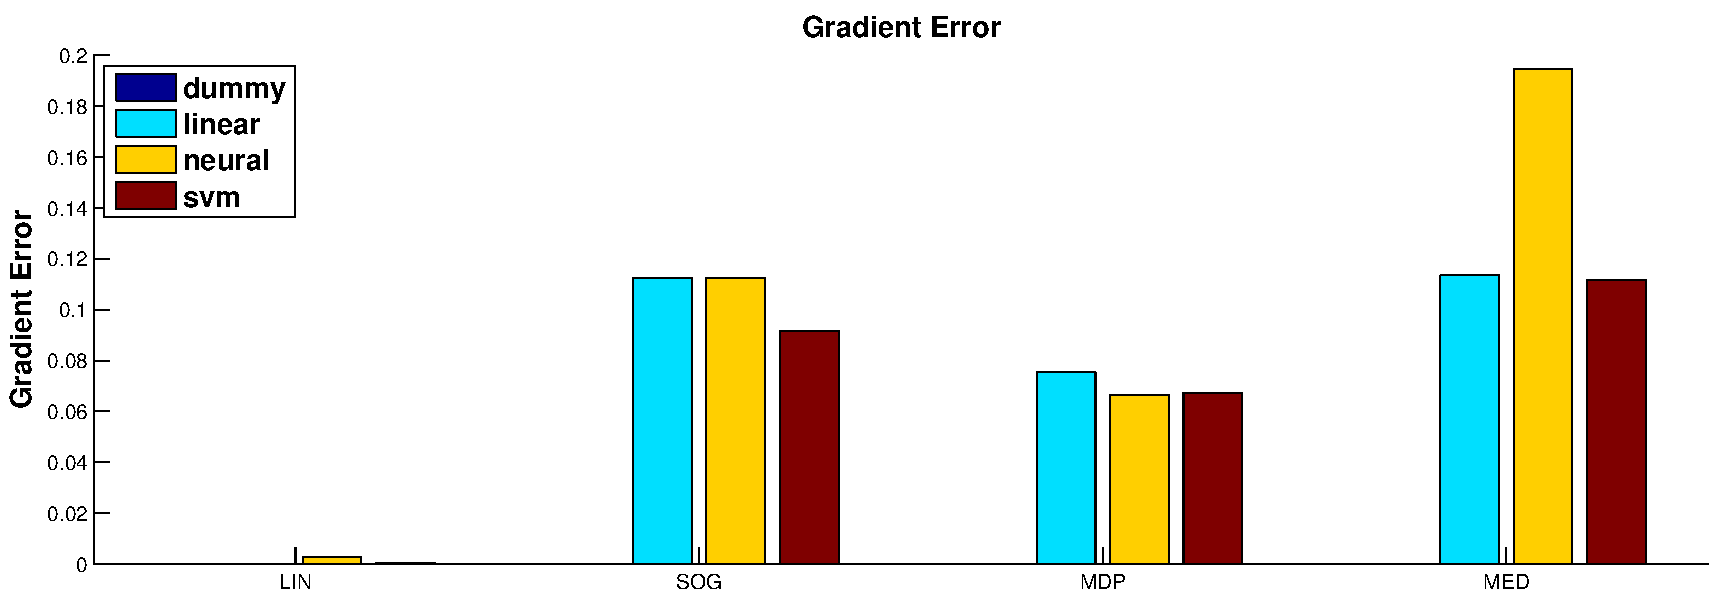
\includegraphics[width=0.8\textwidth]{images/results_grad_rmse}
  \caption{Average gradient error by approximation strategy. }
  \label{fig:results_grad_rmse}
\end{figure}

\subsection{Performance}

Figure~\ref{fig:results_train_time} shows the time required to train each approximating function, a value which may alternatively be considered the compilation latency. The linear approximator takes only on the order of a second, while the neural network and SVM models require more extensive training periods.

\begin{figure}
  \centering
  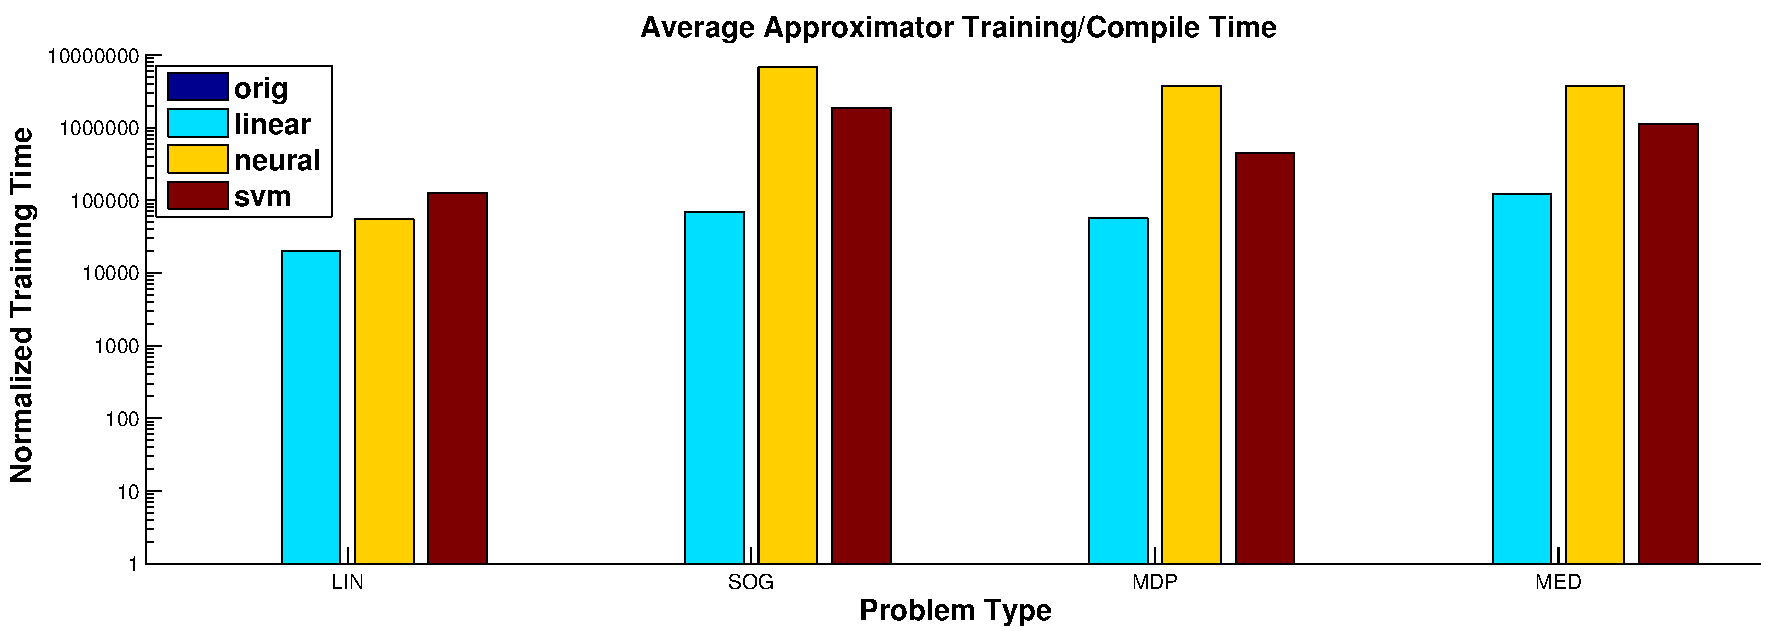
\includegraphics[width=0.8\textwidth]{images/results_train_time}
  \caption{Time required to train/compile each approximator}
  \label{fig:results_train_time}
\end{figure}

Finally, the runtime execution and number of execution instructions are featured in \ref{fig:results_run_time}. Note that, in some cases, these two performance metrics diverge, indicating that dynamic instruction counts are not always a good predictor of runtime efficiency. In particular, the linear approximator demonstrates consistently minimal dynamic instruction counts, but this does not equate to the highest wall clock performance for the MDP and MED problem types, where both the neural network and SVM approximators prevail.

Note also that the approximated functions only showed better runtime performance than the original function for the MDP problem type, which is an intensive value iteration over a relatively large state space. In all three other problem types, the approximators in fact show significant slowdowns relative to the original function. We address this observation in Section~\ref{sec:project_notes}.

\begin{figure}
  \centering
  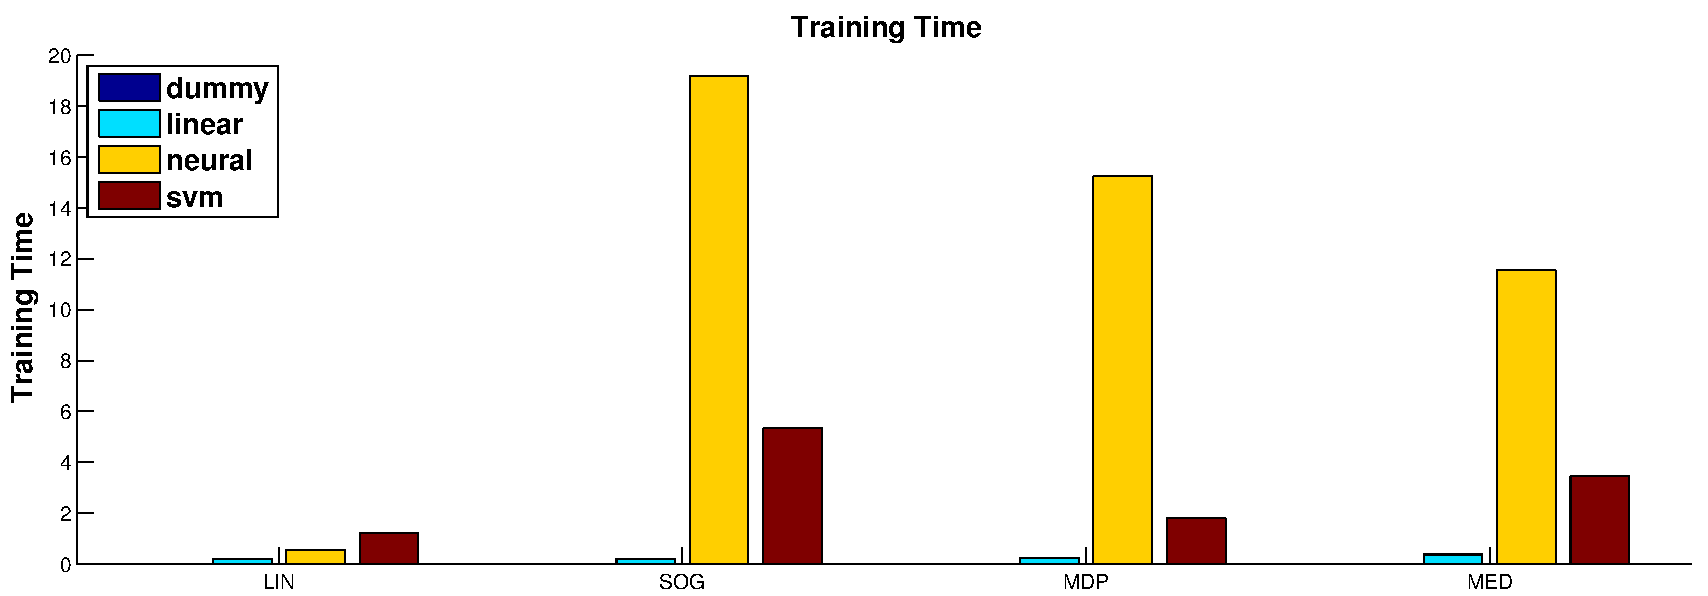
\includegraphics[width=0.8\textwidth]{images/results_run_time}
  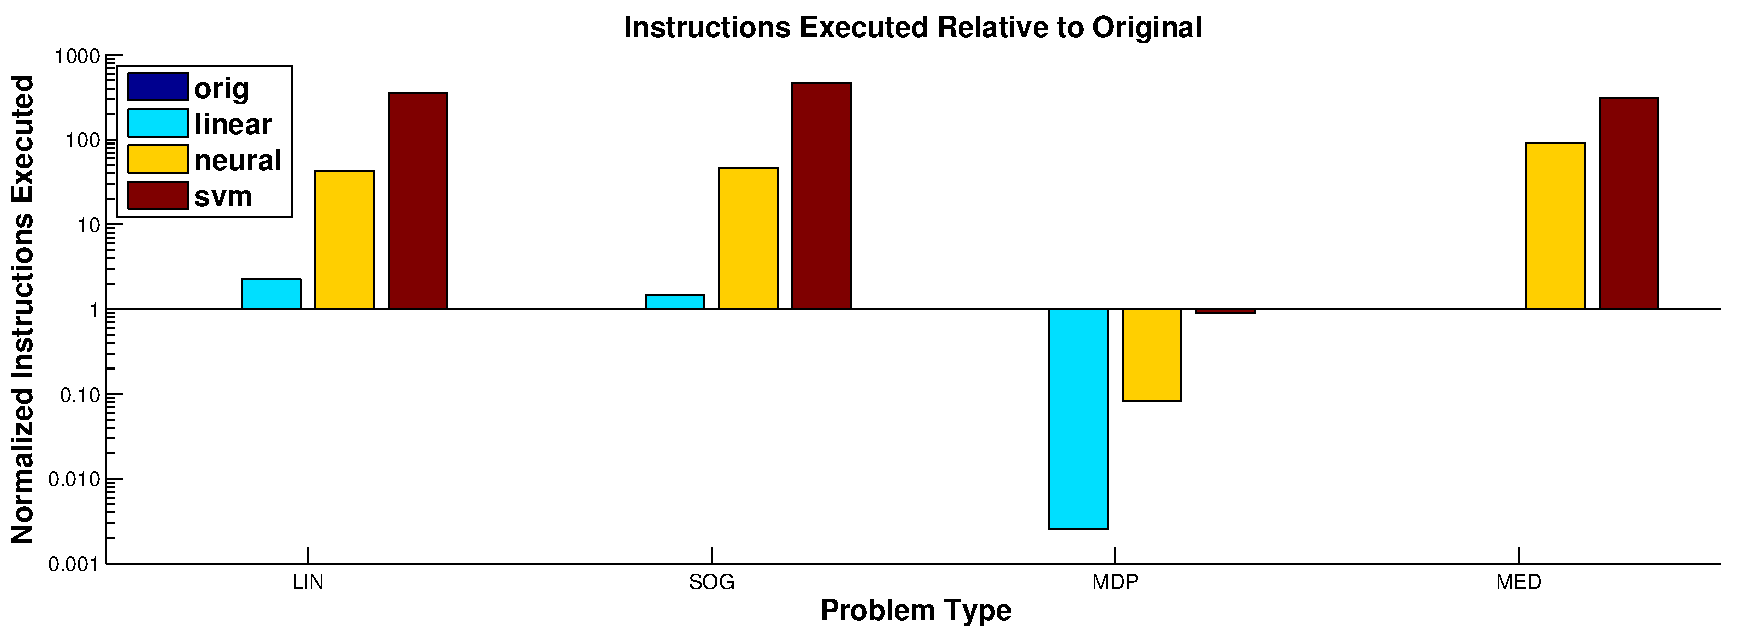
\includegraphics[width=0.8\textwidth]{images/results_instructions}
  \caption{Average function runtime (top) and number of instructions executed (bottom) by approximation strategy (log scales)}
  \label{fig:results_run_time}
\end{figure}

\section{Project Notes}
\label{sec:project_notes}

Specialized hardware is an important factor when it comes to execution efficiency, and one to which we did not have access while working on this project. Esmaeilzadeh~\cite{Esmaeilzadeh12} used a specially-designed ASIC to enable values in neural networks to be computed extremely quickly; since we were limited to software solutions, our approximators were typically slower than the original code, often significantly. However, the hope is that, for any of the approximator types, it would be possible to implement that approximator efficiently in hardware, whereas it would be much more difficult to implement similar hardware for the original general functions.

\bibliographystyle{ieeetr}
\bibliography{sources}

\end{document}
